\newpage
% \setcounter{page}{1} % only for draft purpose to keep page count on track
\section{Pulsar Searching in a Binary System} \label{sec:method-pulsar-searching}

As outlined in \cref{sec:prelude} the study of redback pulsars has a multitude of science cases. However, the number of known redback is small, in searching for new redback pulsars allows for further inquiry into the nature of the subclass. The search usually begins with the selection of potential candidates from large-scale surveys carried out by optical, X-ray and $\gamma$-ray observatories. Candidates are determined based on the flaring exhibited at these shorter wavelengths, then followed up using radio telescopes. Work to date has been to perform follow-up radio observations of Redback candidates to attempt to confirm radio emission and further compliment prior multi-wavelength studies. \

The \textit{Fermi} Large Area Telescope (LAT) provides the most candidates as the related $\gamma$-ray emission are not subject to the same limitations as other detection methods \citep{ray_radio_2012}. Both candidates observed so far as part of this project are two \textit{Fermi} candidates 1FGL J0523.5-2529 and 4FGL J2054.2+6904. 

\subsection{Observation Campaigns}

J0523 was the first observed candidate and was observed using the Ultra-Wide-Bandwidth, Low Frequency Receiver (UWL)\footnote{The UWL operates from 704 to 4032 MHz (40 - 7 cm)} on the Parkes Murriyang telescope in New South Wales. Published studies from \cite{strader_1fgl_2014} and \cite{halpern_luminous_2022} provide the orbital period, companion's radial velocity and distance measurements for the system. Each of these factors are important in determining the observation and search strategy. \ 

For the pulsar to be detected the radio emission from the poles must be visible to the observer plane of view and the beam must not be obscured by the companion star. The orbital phase can be easily calculated from the periodic emission in the optical as demonstrated in \cref{fig: velocities} using the following equation, 

\begin{equation}
    \phi = \frac{t - T_0}{P_{\text{orb}}}
    \label{eq: orbital phase}
\end{equation}

At the time of writing 74\% of the orbital phase has been observed, with time approved to observe the remaining orbital phase if the pulsar is not detected. \\

In the case of J2054 less information is known with no accurate phase ephermeris available. A study by \cite{karpova_new_2023} reports the period, companion radius and distance. Over 8 hours of observations have been carried out using I-LOFAR. In this case the entire orbit needs to be covered and blindly searched for radio emission within expected parameter range of a Redback pulsar. Observations with OSMOS, the Ohio State Multi-Object Spectrograph \citep{martini_ohio_2011} are planned to take place in the Summer of 2024 to try and determine the time of ascending orbital phase. 

\begin{figure}[h] %[h!]
    \centering
    \subfloat[\centering]{{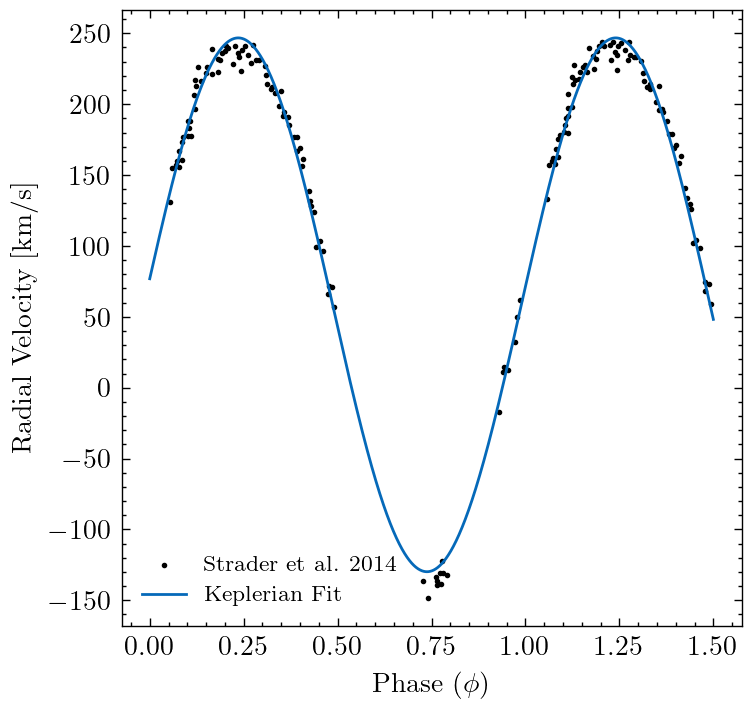
\includegraphics[width = 0.46\textwidth]{figs/radial-velocity.png}}}%
    \qquad
        \subfloat[\centering ]{{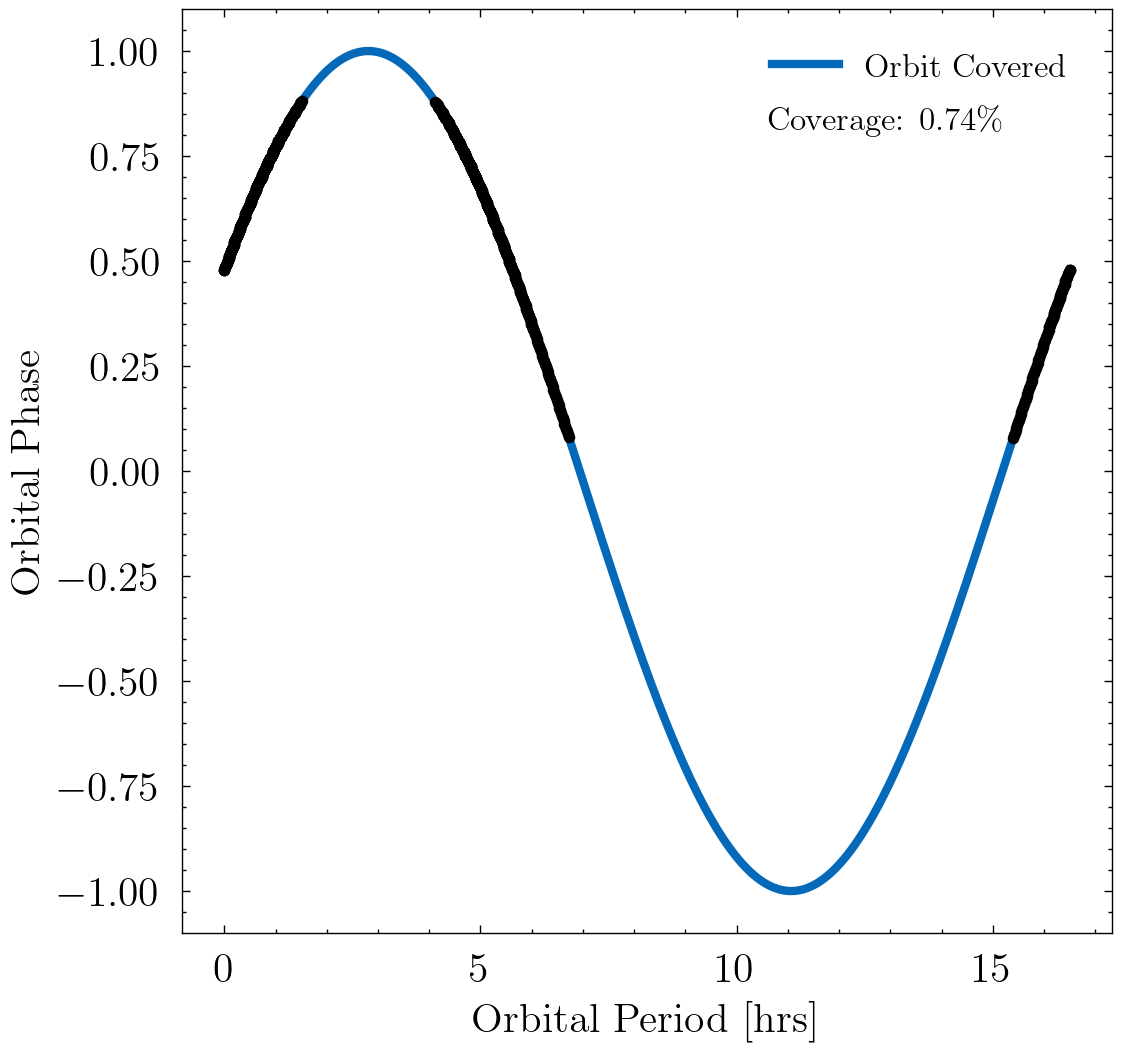
\includegraphics[width=  .46\textwidth]{figs/sine-wave-coverage.png}}}%
    \caption{\textit{(a)} Phased radial velocities observed from the optical counterpart of J0523 with the Keplerian fit plotted on top. \textit{(b)} Observed orbital phase of J0523 with Parkes UWL to date. }%
    \label{fig: velocities}%
\end{figure}

\subsection{Observation Data} \label{sec:method-observation-data}

Observations from radio telescopes typically includes measurements of intensity, frequency, polarization and time. The data is usually stored in a time series format with the intensity and frequency measurements recorded at each time step. The data is usually stored in a  filterbanks (\texttt{.fil}) or .fits file format. The raw voltages are recorded and then processed into usable Stoke I files. 

\subsection{Search Strategy}

A zoo of pulsar software has been developed over the past decades to detect and time pulsars. One of the most commonly used software in the search for binary pulsars is PRESTO \citep{ransom_new_2001}. The search is carried out as illustrated in \cref{fig: presto-work-flow} and due to the large data volumes produced by modern telescopes, the search is carried out in a distributed manner on high performance computing clusters. \\ 

\begin{figure}[h]
    \centering
    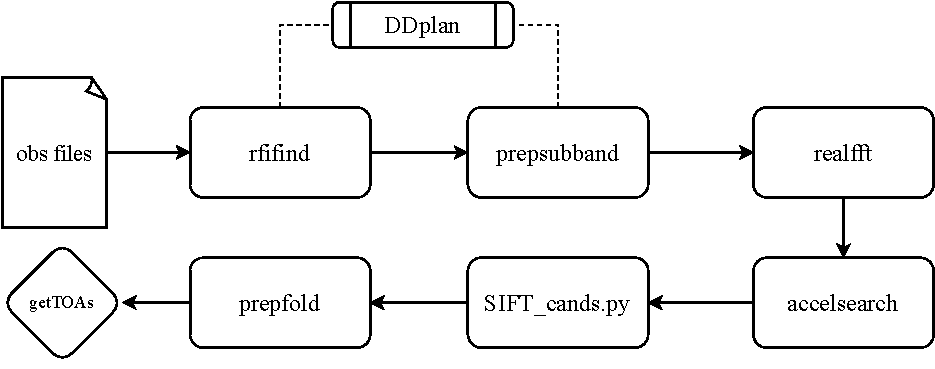
\includegraphics[width = 0.9\textwidth]{figs/presto_pipeline.pdf}
    \caption{Outline of the PRESTO search strategy used to search for binary pulsars.}
    \label{fig: presto-work-flow}
\end{figure}

\subsubsection{RFI Removal}

The first step in nearly all radio observations is to remove Radio Frequency Interference (RFI) from the observations data, this is usually caused by most modern technologies. This is important as artifical signals can mimic period signals associated with pulsar emission. Thus the data must mask frequencies or be clipped in the time domain. This project makes use of \texttt{rfifind} to remove such RFI. 

\texttt{rfifind} which is part of the PRESTO suite searches in both frequency and time domains. It analyses each channel for a specified time integration. Firstly the time domain statitics are computed which consists of the mean and standard deviation of the values in each channel. For blocks where the mean value exceeds $4\sigma$ the block is flagged as RFI. If more than 30\% of the channel is flagged the entire channel is masked completely and replaced with a median constant band-pass value. An example of a mask produced by \texttt{rfifind} is shown in \cref{fig: rfifindexample}. 

\subsubsection{Incoherent Dedispersion}

Following the masking of all observation files the next step is to incoherently dedisperse the data. This is done to remove the effects of dispersion caused by the interstellar medium as discussed in \cref{sec:DispersionMeasure}. Failure to de-disperse data broadens potential pulse profiles and significantly reduces the signal to noise ratio. \Cref{fig: DM_pulse_example} shows an example of pulse dispersion. Incoherent dedispersion is carried out by splitting the data into sub-bands and then shifting the data in time to correct for the dedispersion. 


\begin{figure}
    \centering
    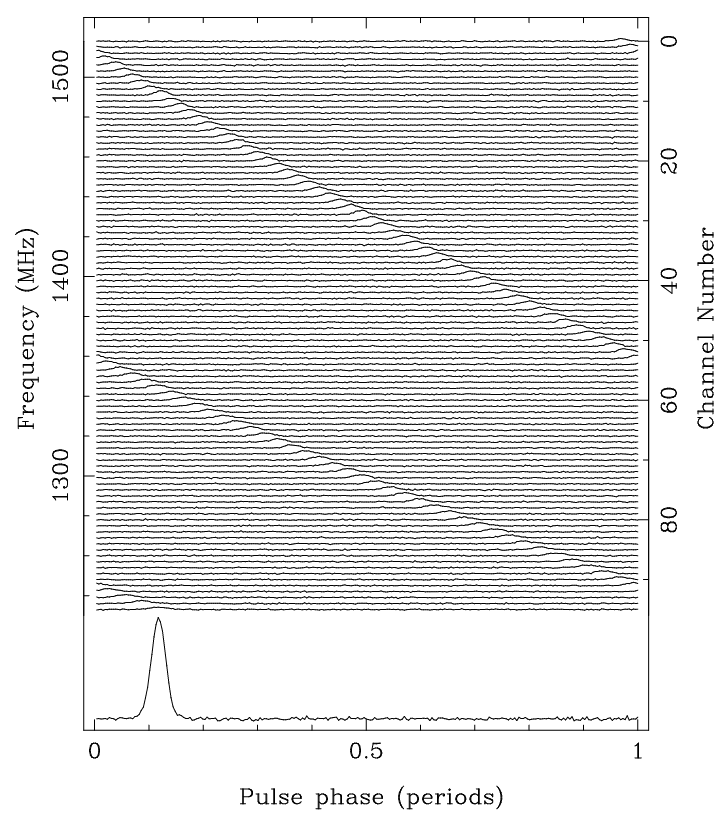
\includegraphics[width = 0.6\textwidth]{figs/DM_pulse_example.png}
    \caption{Example of a dispersion pulses of 128 ms pulsar B1356-60, which has a dispersion measure of 295 pc cm$^{-3}$. Figure from \citet[p.~20]{pulsar_handbook}.}
    \label{fig: DM_pulse_example}
\end{figure}

When correcting for dispersion it is important to consider the possible range of DMs that the pulsar could exhibit. The DM can be estimated through the use of density electron models such as \cite{cordes_ne2001i_2003} and \cite{yao_new_2017}. However when dedisperseing the data it inherently induces smearing in the data. There are four types of smearing that need to be accounted for and characterized by the following equation, 

\begin{equation}
    \tau_{\text{total}} = \sqrt{\tau_{\text{samp}}^2 + \tau_{\text{sub}}^2 + \tau_{\text{BW}}^2 + \tau_{\text{chan}}^2}
\end{equation}

Where $\tau_\text{chan}$ is the channel smearing, $\tau_\text{samp}$ is the sample time, $\tau_\text{sub}$is the subband smearing and $\tau_\text{BW}$ is the bandwidth smearing. Coherent dedispersion entails mitigating dispersion effects by employing the complex conjugate of the interstellar medium's transfer function to deconvolve the data before undergoing filterbanking. By adopting this approach, the original instrumental or Nyquist time resolution is preserved, ensuring high sensitivity and minimal smearing, thereby facilitating the detection of millisecond pulsars \citep{hankins_pulsar_1975}. 



\begin{figure}
    \centering
    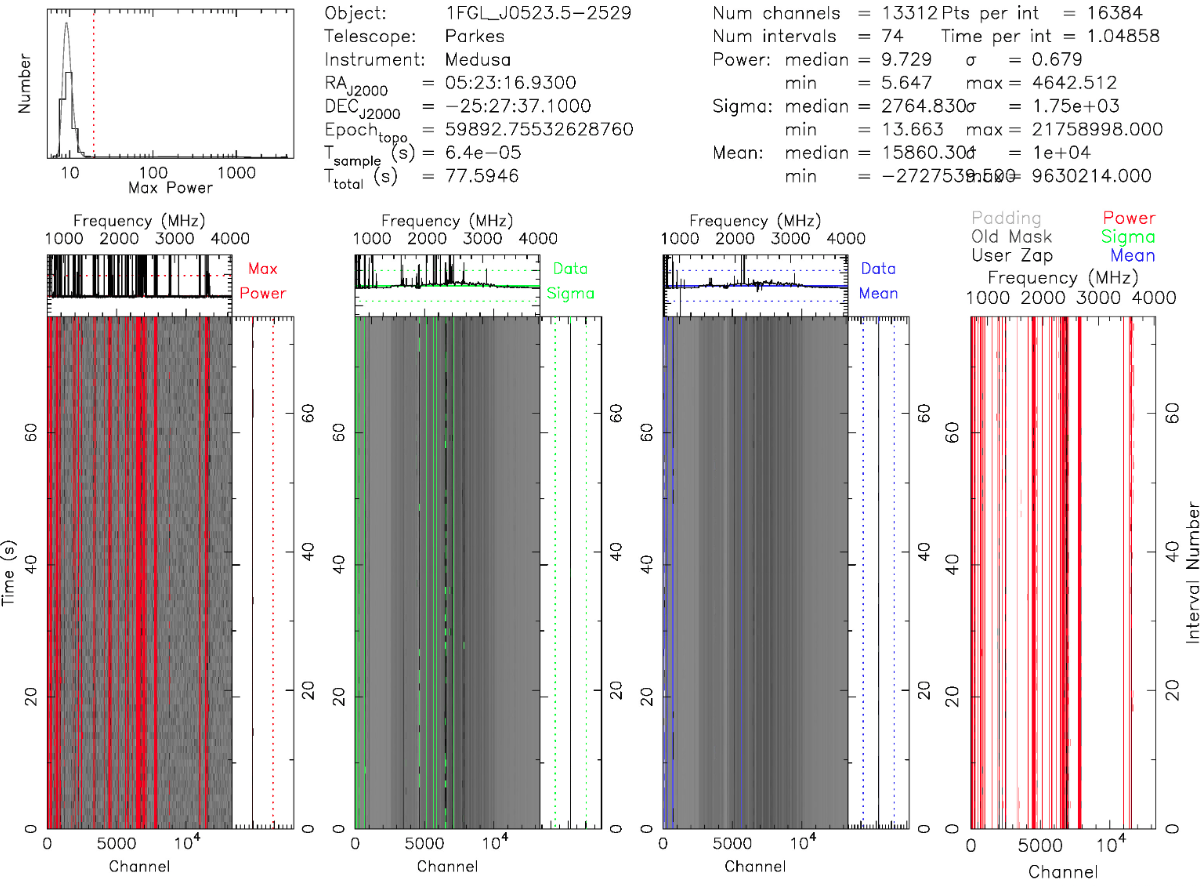
\includegraphics[width = 0.8\textwidth]{figs/rfifindexample.png}
    \caption{Example of RFI removal using \texttt{rfifind} on a 77 second observation of J0523. The upper left panels shows the max power profile of the RFI detected. The bottom most left panel show the max power, the second panel to the right shows the $\sigma$, the third panel shows the mean and the right most panel is the recommended mask with all panels plotted.}
    \label{fig: rfifindexample}
\end{figure}

\subsubsection{Fast Fourier Transform}

The data is needs to be transformed into the frequency domain to search for periodic signals. This is commonly done with a Discrete Fourier Transform (DFT) in pulsar astronomy and computationally carried out using a Fast Fourier Transform (FFT). For a time series, $S_j$ of a given length of $N$ it is necessary to convert the time series into the barycentric frame of reference. The barycentric frame if reference point is centered on the mass of the solar system. \\ The $k$th Fourier component of the time series is described in \citet[pp.~132--134]{pulsar_handbook} as,

\begin{equation}
    \mathcal{F}_k = \sum_{j=0}^{N-1} S_j \exp\left(-2\pi \sqrt{-1} \frac{jk}{N}\right)
\end{equation}

To complete this computation it requires $N^2$ floating point operations. However, if a FFT operation is employed the number of operations is reduced to $N \log_2 N$ for a time series of length $N$. Since the time series data are real numbers symmetry can be exploited as the DFT is symmetric about the Nyquist frequency, $\nu_{\text{Nyq}} = 1/(2 t_{\text{samp}})$. For any frequencies higher than the $\nu_{\text{Nyq}}$ the complex conjucate is the same as the corresponding lower half of the frequency.

On the software side this is carried out with the \texttt{realfft} function in PRESTO. This result intakes the dedisperesed sub-bands and returns the power spectrum of the data. At this point the data is in a state to be searched for periodic signals.

\subsubsection{Accelration Searching}

Searching for binary pulsars requires a slightly different approach as the motion of the system causes the observed pulse frequency to smear across the Fourier bins \citep{ng_high_2015}, in turn this reduces the sensitivity of the search. A solution to this is to split up the search into smaller time intervals and assume that the radial velocity is a constant on this time scale. This can be shown to be a good approximation for $P_b/10$. \\ 
The spin frequency, $f_{\text{spin}}$ and the time of pulse emission, $t_{\text{pulse}}$ the pulsar's phase can be expressed as, $\phi_p = f_{\text{spin}}t_{\text{pulse}}$. Moreover, the pulse time can be expressed as the time of arrival from the pulsar, $d(t_0)$, 

\begin{equation}
    t_{\text{pulse}} = t_0 - \frac{d(t_0)}{c}
\end{equation}

thus the phase can be expressed as,

\begin{align}
    \phi_p = & f_{\text{spin}}\left[ t_0 - \frac{d(t_0)}{c}\right] \\ 
    = & f_\text{spin} \left[ t_0 - \frac{a \sin i}{c} \sin \left[ \frac{2 \pi (t - t_{\text{asc}})}{P_B} \right] \right]
\end{align}

where $a$ is the semi-major axis, $i$ is the inclination angle, $t_{\text{asc}}$ is the time of ascending node and $P_B$ is the orbital period. A Taylor expansion can be used to $\sin x$ around $x = a$ such that, 

\begin{equation}
    \sin (x) \simeq   \sin (a) + \cos (a)(x - a) - \frac{\sin (a)}{2!}(x - a)^2 - \frac{\cos (a)}{3!}(x - a)^3 + \ldots
\end{equation}

Therefore the phase of the pulsar with a constant spin down rate can be expressed as, 

\begin{equation}
  \phi(t) = f^1 t_0 + \frac{\dot f}{2} (t - t_0)^2 + \frac{\ddot f}{6} (t - t_0)^3 + \ldots 
\end{equation}

Matching co-effcients between the the full Taylor expansion and the phase expression for the pulsar gives the following relation, $\dot f/2 = f_{\text{spin}} \frac{a \sin i}{c} A$. Where $A$ is represents all the terms in the expansion. The final simplified expression works out to be, 

\begin{equation}
    \dot f = f_\text{spin} \frac{4 \pi^2 a \sin i }{cP^2_B} \sin \left[ \frac{2 \pi (t - t_{\text{asc}})}{P_B} \right]
\end{equation}

Thus over a small enough time period spin-down is approximately constant.

\begin{equation}
    \frac{k_2 P_B}{2 \pi q} = a \sin i   
    \label{eq:constant_accel}
\end{equation}

Where $k_2$ is the radial velocity semi-amplitude, $P_B$ is the orbital period and $q$ is the mass ratio.

Searching is carried out using \texttt{accelsearch} which searches the FFT time series for period emissions by summing the highest Fourier frequency derivative. The number of bins that this signal is smeared is given by the acceleration parameter \citep{ransom_new_2001}, 

\begin{equation}
    z \simeq \dot f T^2_{\text{obs}}
\end{equation}

Where $T_{\text{obs}}$ is the length of the observation. The search is carried out over a range of accelerations which can be based on \cref{eq:constant_accel} if the physical quantities are known. A list of the known orbital parameters for the two candidates is given in \cref{tab:orbital-parameters} along with resultant z values.
 
\begin{table}[H]
    \centering
    \begin{tabular}{c|cccccc}
        \hline
        Candidate & $P_{\text{orb}}$ (days) & $k_2$ (kms$^{-1}$) & $a \sin i$ (s) & $e$ & $q$ & z\\
        \hline
        J0523.5-2529 & 0.68813 & 190.3 & 0.359 & 0.040 & $0.61 \pm 0.06$ & $3.56 - 335.36$ \\
        J2054 & 0.31111 & \nodata  & \nodata & \nodata & \nodata &\nodata \\
        \hline \hline 
    \end{tabular}
    \caption{Orbital parameters of the two candidates. Values for J0523 are taken from \cite{strader_1fgl_2014} and \cite{halpern_luminous_2022}. Values for J2054 are taken from \cite{karpova_new_2023}.}
    \label{tab:orbital-parameters}
\end{table}

In cases where the orbital parameters are not known the search is carried out over a range of accelerations from 0 to 200, and even in the case where the value exceeds 200, this is left as a cap on the search. The reason that the search is not carried out over the entire range is due to the computational cost and is often not necessary with accelerations above 200 starting to exhibit a non-linear relationship as stated in \citet{ransom_new_2001}. Once the search is carried out the results are outputted in the form of candidates with estimates on DM, S/N, period and frequencies. 

\subsubsection{Folding} \label{sec:folding}

Pulsar folding is a technique commonly used when the pulses are not bright enough to be clearly visible in the observed time series. The term folding comes from the fact that the time series is folded on itself by some trial period of the pulsar, this is illustrated in \cref{fig: folding}. 
% \begin{equation}
%      = n_{\text{samp}} \cdot n_{\text{DM}} \cdot n_\text{Accel} \cdot n_{\text{Harmonics}}
% \end{equation}

\begin{figure}
    \centering
    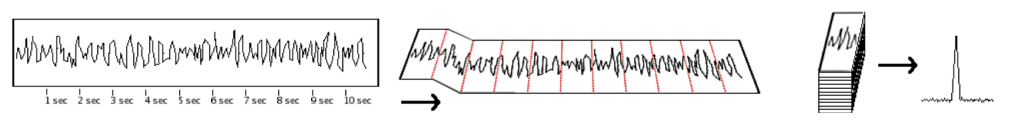
\includegraphics[width = 0.9\textwidth]{figs/folding.png}
    \caption{Adapted illustration from \cite{folding_picture} of the folding process. The left panel shows the observed time series, the middle panel shows the folded time series and the right panel shows the summed pulse profile.}
    \label{fig: folding}
\end{figure}

Using a routine called \texttt{prepfold} each of the candidates over the noise floor are folded with each candidate examined by eye for possible positive pulsar detection. An example of this is shown in \cref{fig: prepfold}. This plot contains integrated pulse profile, time series plot and sub-band plot. It also shows DM, $P$ and $\dot P$ plots as a function of reduced $\chi^2$ values. Each of these plots must be sifted through by eye. A pulsar will exhibit a single high S/N peak in the DM, $P$ and $\dot P$ plots similar to those shown in the plot if its a positive candidate. 

\begin{figure}
    \centering
    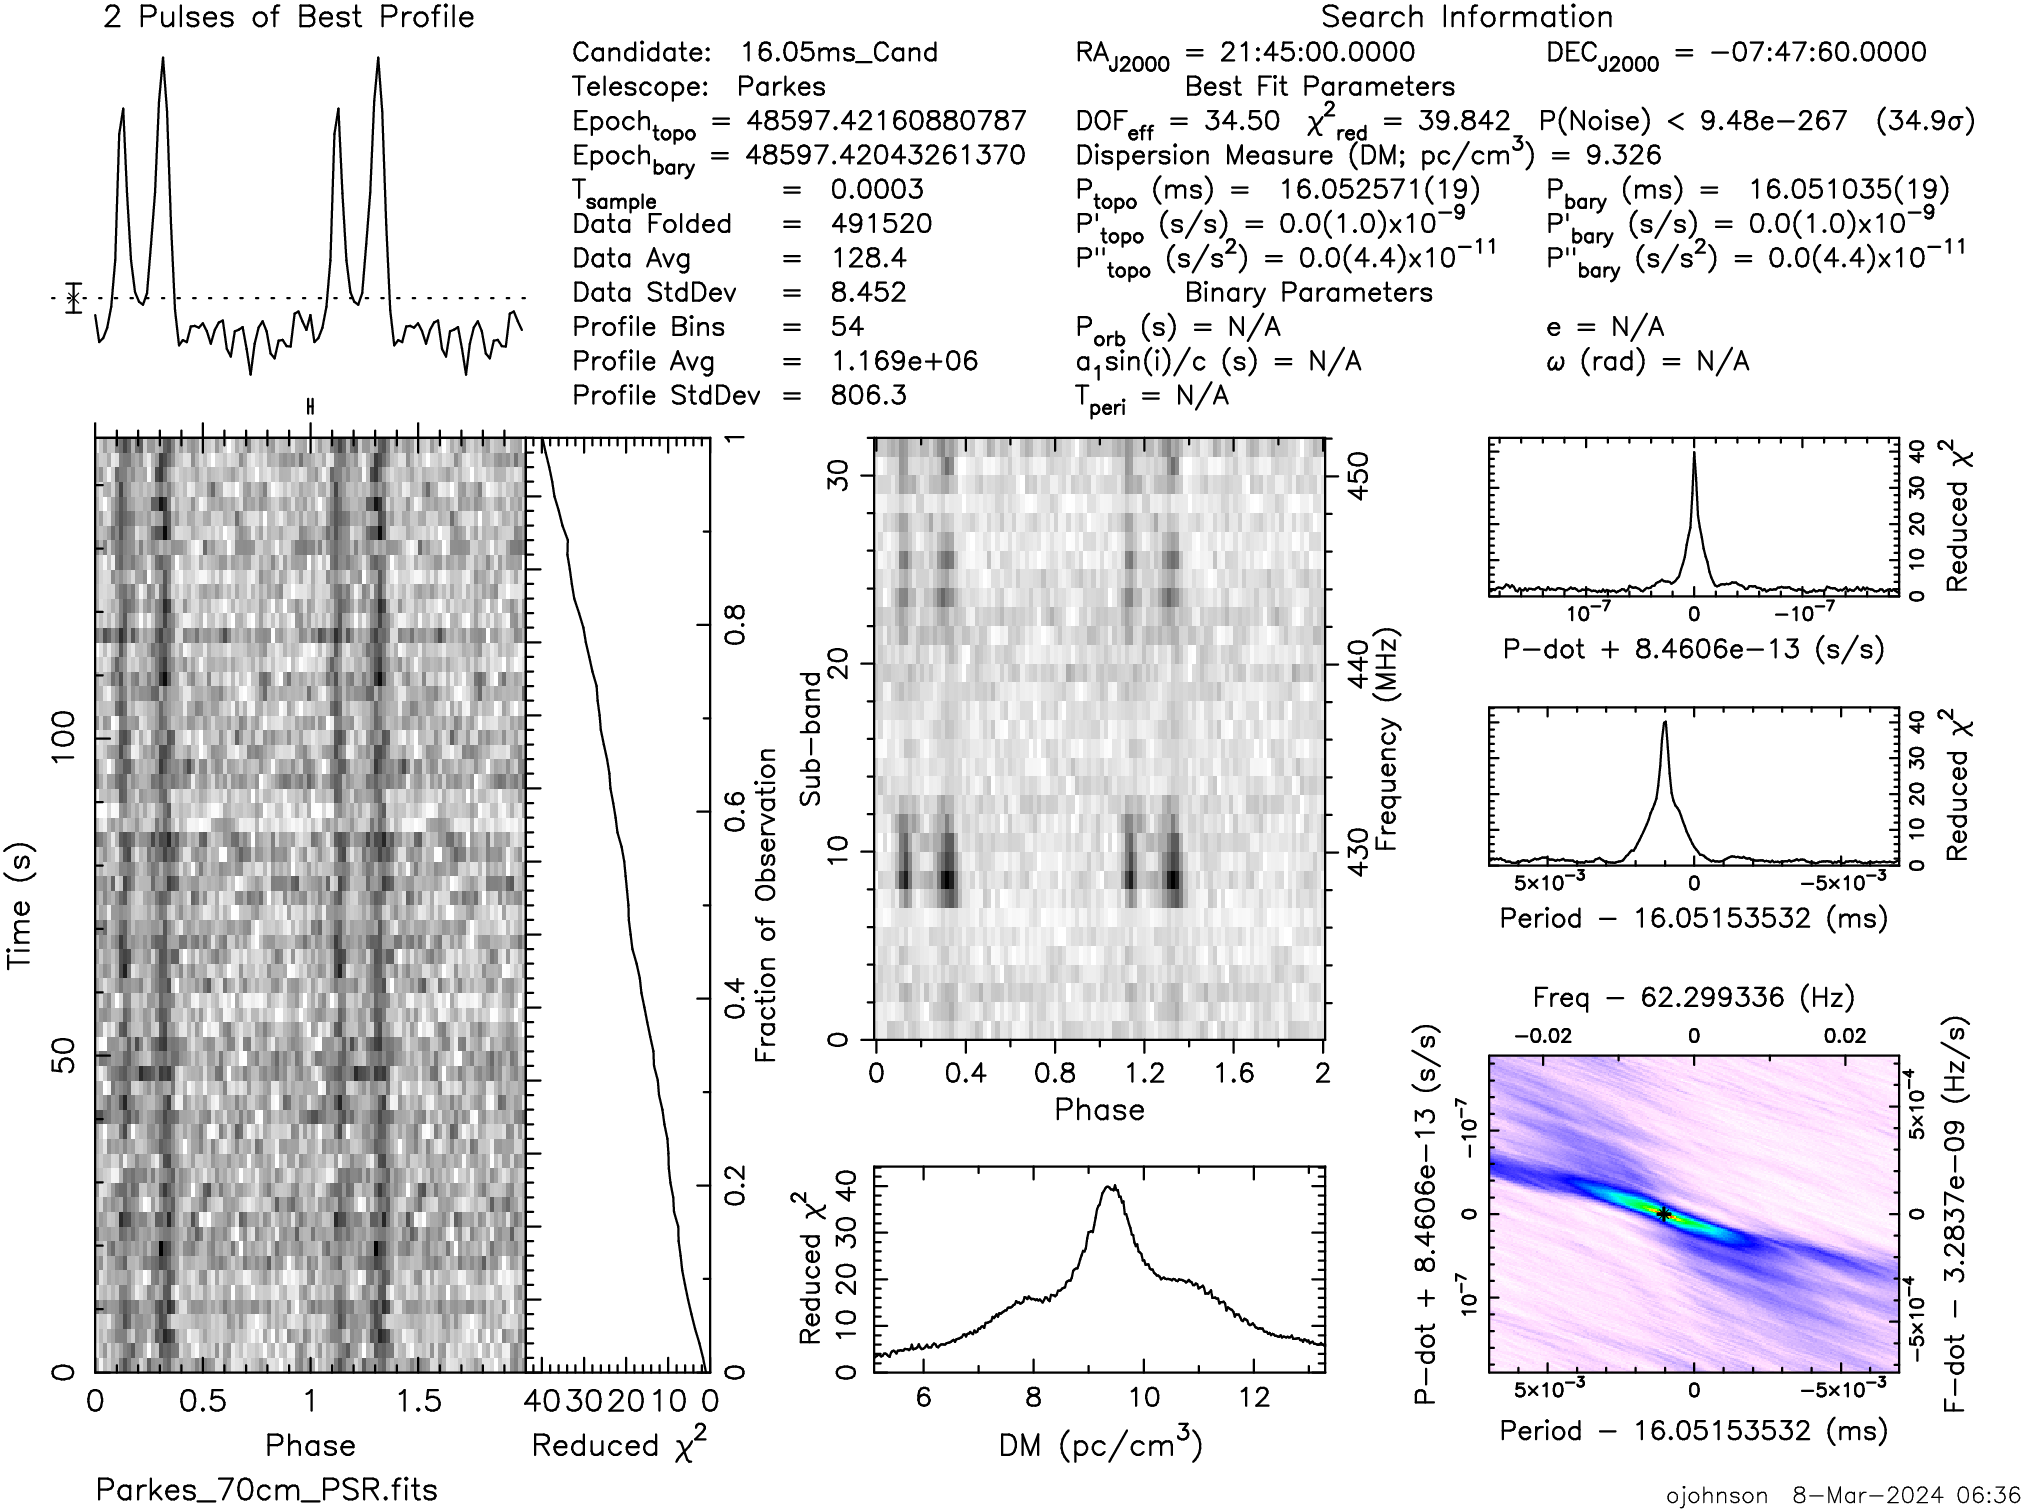
\includegraphics[width = 0.9\textwidth]{figs/pulsar-cand.png}
    \caption{Example of a \texttt{prepfold} plot for J2145-0750 using described pipeline.}
    \label{fig: prepfold}
\end{figure}

